\documentclass[usenames,dvipsnames,tikz]{standalone}
\usepackage{xcolor}
\colorlet{tBlue}{RoyalBlue!35!Cerulean}
\colorlet{tRed}{Red}
\usepackage{tikz}
\usepackage{standalone}
\begin{document}
	
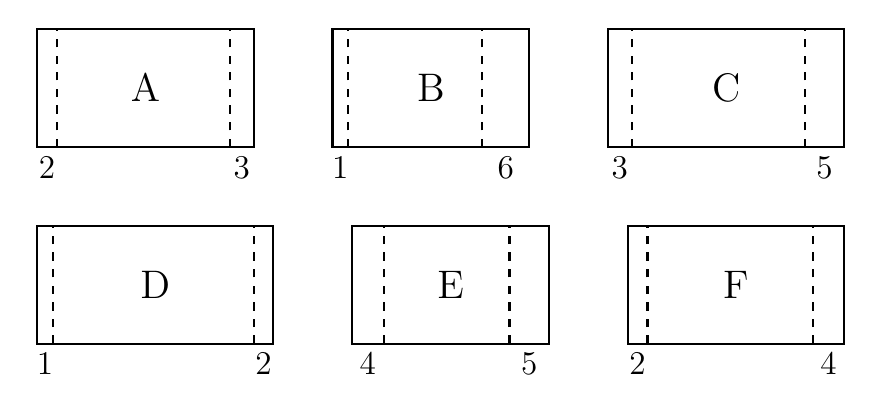
\begin{tikzpicture}
%\draw [help lines] (-1,-2) grid (11,5);

\draw [thick] (0,2.5) rectangle (2.75,4); % A (2,3)
\draw [thick, dashed] (0.25,2.5) -- (0.25,4);
\draw [thick, dashed] (2.45,2.5) -- (2.45,4);
\node [below] at (0.125, 2.5) {\large{2}};
\node [below] at (2.6, 2.5) {\large{3}};
\node at (1.375,3.25) {\Large{A}};

\draw [thick] (3.75,2.5) rectangle (6.25,4); % B (1,6)
\draw [thick, dashed] (3.95,2.5) -- (3.95,4);
\draw [thick, dashed] (5.65,2.5) -- (5.65,4);
\node [below] at (3.85, 2.5) {\large{1}};
\node [below] at (5.95, 2.5) {\large{6}};
\node at (5,3.25) {\Large{B}};

\draw [thick] (7.25,2.5) rectangle (10.25,4); % C (3,5)
\draw [thick, dashed] (7.55,2.5) -- (7.55,4);
\draw [thick, dashed] (9.75,2.5) -- (9.75,4);
\node [below] at (7.4, 2.5) {\large{3}};
\node [below] at (10, 2.5) {\large{5}};
\node at (8.75,3.25) {\Large{C}};

\draw [thick] (0,0) rectangle (3,1.5); % D (1,2)
\draw [thick, dashed] (0.2,0) -- (0.2,1.5);
\draw [thick, dashed] (2.75,0) -- (2.75,1.5);
\node [below] at (0.1, 0) {\large{1}};
\node [below] at (2.875, 0) {\large{2}};
\node at (1.5,0.75) {\Large{D}};

\draw [thick] (4,0) rectangle (6.5,1.5); % E (4,5)
\draw [thick, dashed] (4.4,0) -- (4.4,1.5);
\draw [thick, dashed] (6,0) -- (6,1.5);
\node [below] at (4.2, 0) {\large{4}};
\node [below] at (6.25, 0) {\large{5}};
\node at (5.25,0.75) {\Large{E}};

\draw [thick] (7.5,0) rectangle (10.25,1.5); % F (2,4)
\draw [thick, dashed] (7.75,0) -- (7.75,1.5);
\draw [thick, dashed] (9.85,0) -- (9.85,1.5);
\node [below] at (7.625, 0) {\large{2}};
\node [below] at (10.05, 0) {\large{4}};
\node at (8.875,0.75) {\Large{F}};






\end{tikzpicture}
\end{document}